On a representative series, all four pipelines produce events with content-addressed identifiers and nonempty provenance. The witness passes a strict JSON round trip. Complete verification recomputes strict candidates, reproduces the visible set, rematerializes \code{SELECT} rows, and verifies their fingerprint and the row at the claimed rank. Alterations of a configuration, event, occurrence manifest, projected manifest, projected row, policy, tolerance, or projector are rejected. All eleven time units and a high-precision duration pass the complete chain.

\begin{table}[H]
\centering
\caption{Provenance validation on the representative series.}
\label{tab:provenance-validation}
\small
\begin{tabular}{lrrrr}
\toprule
Pipeline & Events & With ID & With provenance & Mean nodes \\
\midrule
First difference & 105 & 105 & 105 & 1.00 \\
Single-scale DoG & 50 & 50 & 50 & 1.00 \\
Multiscale maxima & 48 & 48 & 48 & 3.40 \\
Maximum lines & 52 & 52 & 52 & 4.15 \\
\bottomrule
\end{tabular}
\end{table}

\subsection{Microbenchmark Separated from Correctness Validation}

Functional correctness is checked by \path{run_validation_fast.sh}; the heavier microbenchmark has its own command, \path{run_microbenchmark.sh}. This separation prevents a continuous-integration check from depending on relations containing 10,000 events. The executed matrix is recorded in \path{results/compiler_microbenchmark_protocol_v7.json}. For 100, 500, and 1,000 events, patterns of two, three, and four atoms are measured under narrow gaps $[2,8]$ and wide gaps $[2,30]$. At 3,000 events, all three pattern lengths are executed for narrow gaps, but only two atoms for wide gaps. At 10,000 events, only two-atom plans are executed in both regimes. The study reports median, P05--P95, and output cardinality. The measurements characterize the Python prototype and are neither a memory benchmark nor a comparison with an industrial DBMS or CEP engine.

\begin{figure}[H]
\centering
\begin{subfigure}{0.48\textwidth}
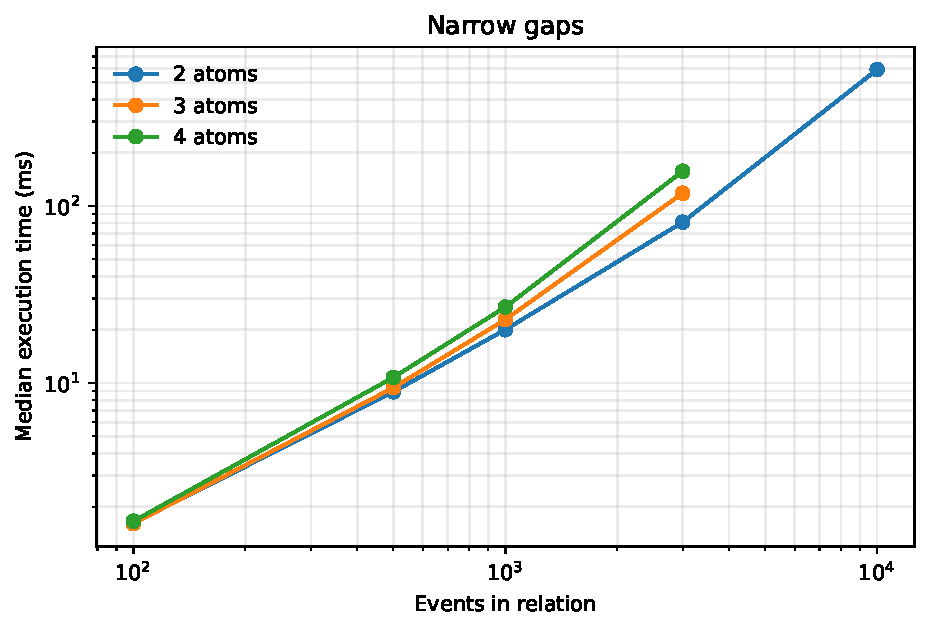
\includegraphics[width=\textwidth]{figures/compiler_microbenchmark_narrow_en.pdf}
\caption{Narrow gaps.}
\end{subfigure}
\hfill
\begin{subfigure}{0.48\textwidth}
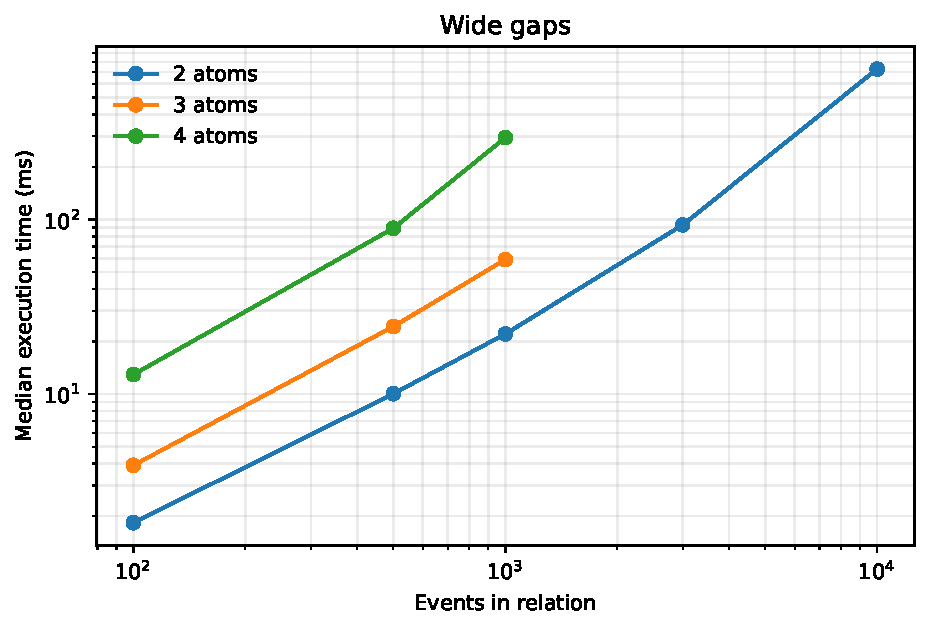
\includegraphics[width=\textwidth]{figures/compiler_microbenchmark_wide_en.pdf}
\caption{Wide gaps.}
\end{subfigure}
\caption{Scaling behavior of the temporal-join plan.}
\label{fig:microbenchmark}
\end{figure}

\section{Synthetic Benchmark of Extraction Pipelines}

\subsection{Corpus, Split, and Patterns}

Six hundred daily series of 365 points are generated with seeds $91000,\ldots,91599$. The first 180 are used exclusively to calibrate one threshold per pipeline and query; the remaining 420 form an evaluation split separate from calibration. Noise levels $\sigma\in\{6,12,20\}$ are balanced.

Each series combines a level $U(160,260)$, a slope $U(-0.05,0.08)$, a weekly sawtooth
\begin{equation}
 [-42,-24,-10,4,24,52,-6]\times U(0.7,1.3),
\end{equation}
an annual sinusoid with amplitude $U(4,18)$, a beginning- and end-of-month effect $U(5,15)$, and AR(1) noise with coefficient $U(0.15,0.45)$. Each pattern family is selected with probability $0.38$, with local exclusion to reduce overlap. Amplitudes lie in $U(45,95)$, and boundaries may be triangular or trapezoidal.

\begin{figure}[H]
\centering
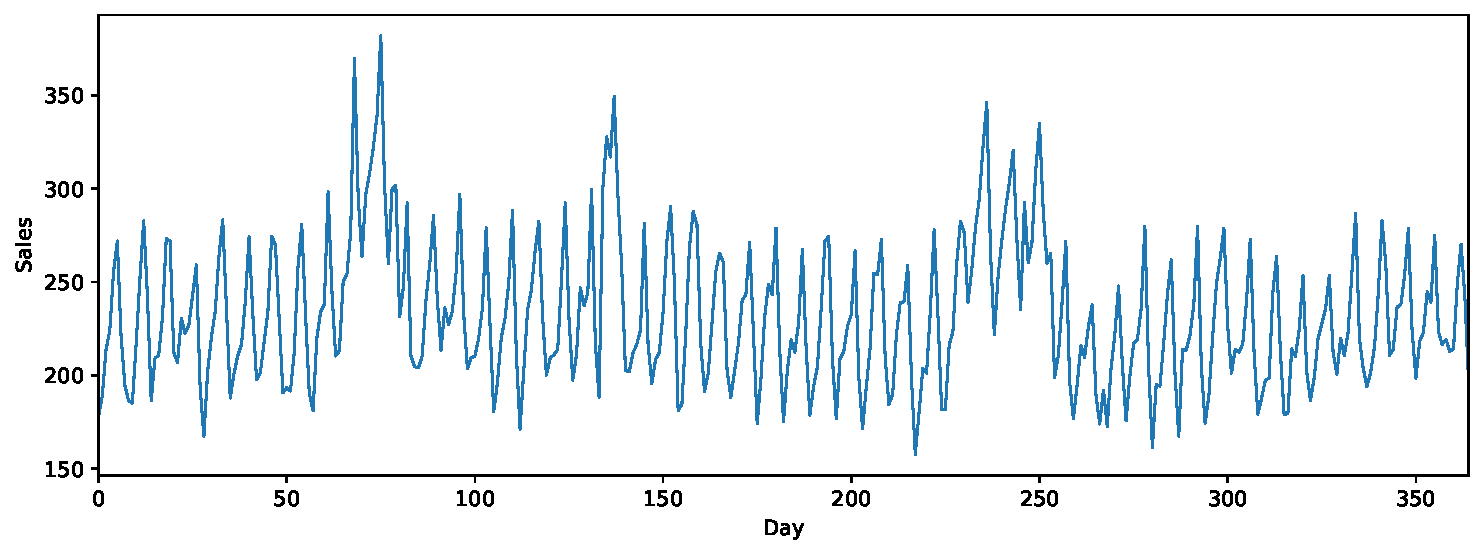
\includegraphics[width=0.96\textwidth]{figures/representative_retail_series_en.pdf}
\caption{Representative synthetic retail-like series with a weekly sawtooth, slow components, autocorrelated noise, and injected transitions.}
\label{fig:retail-example}
\end{figure}

\begin{table}[H]
\centering
\caption{Evaluated morphological queries.}
\label{tab:queries}
\small
\begin{tabularx}{\textwidth}{@{}p{1.1cm}p{5.2cm}X@{}}
\toprule
ID & Expression & Description \\
\midrule
Q1 & $+\xrightarrow{1\text{--}4\,\mathrm{d}}-$ & brief peak \\
Q2 & $+\xrightarrow{8\text{--}14\,\mathrm{d}}-$ & bounded positive episode \\
Q3 & $+\xrightarrow{18\text{--}28\,\mathrm{d}}-$ & long positive episode \\
Q4 & $-\xrightarrow{5\text{--}10\,\mathrm{d}}+$ & temporary trough \\
Q5 & $+\xrightarrow{8\text{--}14\,\mathrm{d}}-\xrightarrow{5\text{--}10\,\mathrm{d}}+$ & rise, fall, rebound \\
Q6 & $+\xrightarrow{1\text{--}4\,\mathrm{d}}-\xrightarrow{3\text{--}10\,\mathrm{d}}+\xrightarrow{1\text{--}4\,\mathrm{d}}-$ & two nearby peaks \\
\bottomrule
\end{tabularx}
\end{table}

\subsection{Comparison, Calibration, and Matching}

The four pipelines share preprocessing, queries, engine, and evaluation protocol, but differ in their extraction rules. The comparison is therefore between complete pipelines. For each pipeline--query pair, a threshold is selected on the calibration split from 100 quantiles constructed from \emph{all} candidate scores. The criterion is F1, with precision and then recall as tie-breakers. Deduplication uses an $L_\infty$ tolerance of two days before calibration and evaluation and is serialized in the protocol.

A prediction and a ground-truth instance of equal length are compatible when their $L_\infty$ distance is at most three days. Optimal bipartite matching first maximizes the number of compatible pairs and then minimizes total boundary error. The 95\% intervals are based on 2,000 paired bootstrap replicates at the series level within the evaluation split, using seed 20260805. They quantify evaluation uncertainty \emph{conditional} on the calibration split and the resulting thresholds; they do not propagate the variability of drawing a new calibration split. Pairwise contrasts are exploratory and not adjusted for multiplicity.

\subsection{Artifact Lineage}

The distributed candidate tables, extraction configurations, and implementation fingerprints are treated as immutable source artifacts. Metric computation, bootstrap intervals, and output manifests are recorded separately from candidate generation. The language and witness contract does not change the extractors, candidate scores, or benchmark labels. The artifact manifest records whether raw candidate generation was rerun and identifies the exact implementation and configuration fingerprints used at each stage.

\subsection{Global Results}

\begin{figure}[H]
\centering
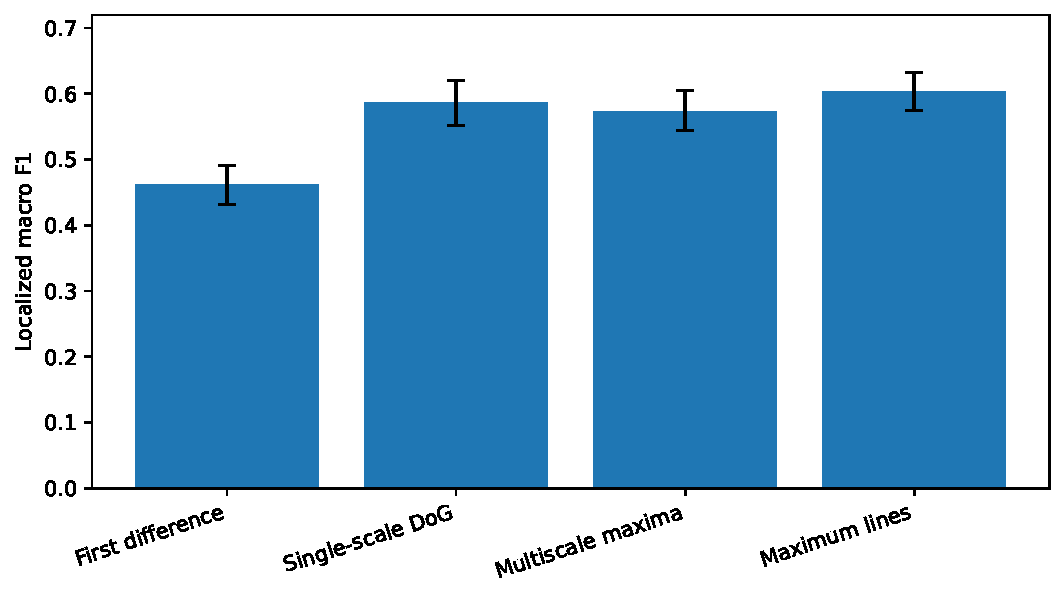
\includegraphics[width=0.82\textwidth]{figures/f1_macro_methods_en.pdf}
\caption{Localized macro F1 on the 420-series evaluation split. The 95\% bootstrap intervals are conditional on fixed calibration.}
\label{fig:global-f1}
\end{figure}

\begin{table}[H]
\centering
\caption{Global pipeline performance. Extraction runtimes come from the archived reference run and are reported descriptively; they are not included in statistical comparisons.}
\label{tab:global-results}
\scriptsize
\begin{tabular*}{\textwidth}{@{\extracolsep{\fill}}lrrrrrr@{}}
\toprule
Pipeline & Macro P & Macro R & Macro F1 [CI] & Micro F1 [CI] & events/series & ms/series \\
\midrule
First difference & .527 & .434 & .462 [.431;.491] & .489 [.458;.518] & 107.0 & 3.468 \\
Single-scale DoG & .735 & .491 & .587 [.552;.620] & .604 [.573;.635] & 46.4 & 1.857 \\
Multiscale maxima & .746 & .475 & .573 [.544;.604] & .592 [.564;.620] & 46.1 & 6.804 \\
Maximum lines & .768 & .503 & \textbf{.604} [.575;.632] & \textbf{.627} [.600;.654] & 49.9 & 12.084 \\
\bottomrule
\end{tabular*}
\end{table}

The runtime environment and provenance are distributed with the reference artifacts. The values locate the computational cost of the prototype; they do not support a statistical performance comparison or characterize a production database system.

On this split, all three wavelet pipelines have higher point estimates than first differences. The paired macro-F1 gain is $+0.125$ for single-scale DoG, $+0.112$ for aggregated maxima, and $+0.142$ for maximum lines; the conditional intervals exclude zero. Maximum lines have the highest global point estimate. Their gain over DoG is $+0.017$, with 95\% CI $[-0.006,0.040]$, so a global advantage is not established. The maximum-lines versus aggregated-maxima contrast is $+0.030$, CI $[0.012,0.049]$, on this split, but it is exploratory, unadjusted, and its point ordering reverses in the additional-seed replication. It does not support a general dominance claim.

\begin{figure}[H]
\centering
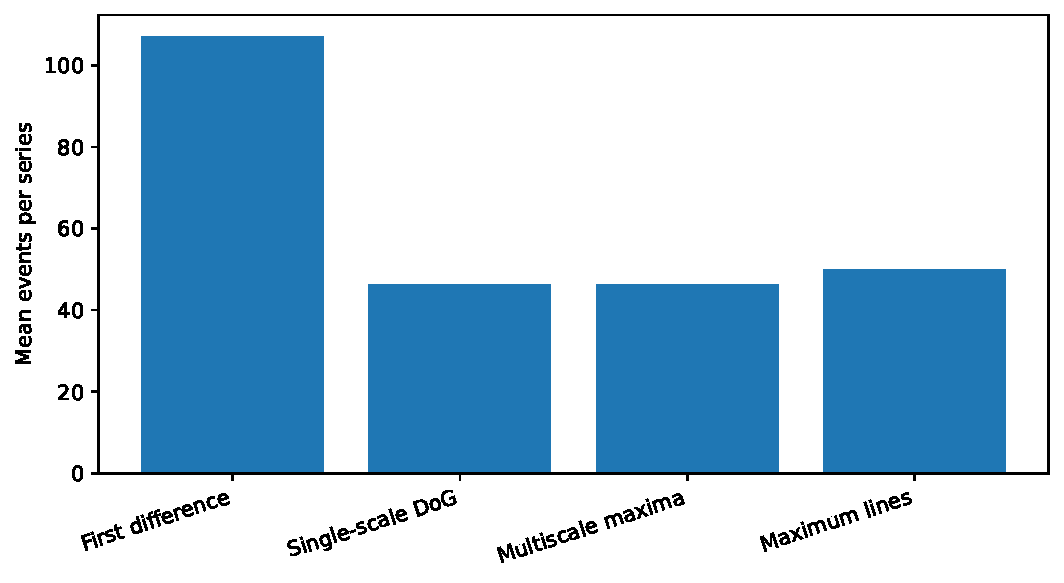
\includegraphics[width=0.76\textwidth]{figures/event_count_methods_en.pdf}
\caption{Mean number of materialized events per series before query execution.}
\label{fig:event-count}
\end{figure}

\subsection{Results by Query and Noise Level}

\begin{figure}[H]
\centering
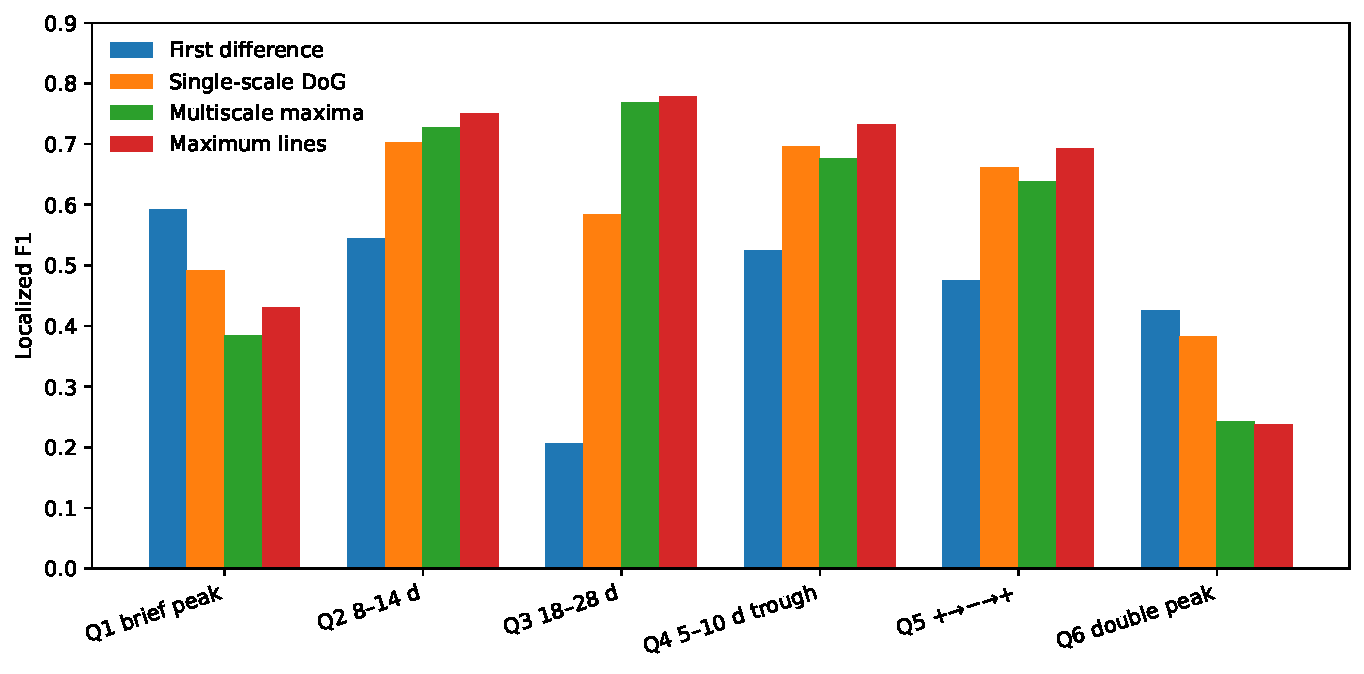
\includegraphics[width=0.98\textwidth]{figures/f1_by_query_en.pdf}
\caption{Localized F1 by query and pipeline.}
\label{fig:query-f1}
\end{figure}

\begin{table}[H]
\centering
\caption{F1 by query family.}
\small
\begin{tabular}{lrrrr}
\toprule
Query & First diff. & Single DoG & Multi. maxima & Max. lines \\
\midrule
Q1 brief peak & \textbf{.592} & .492 & .384 & .430 \\
Q2 8--14 d episode & .544 & .703 & .728 & \textbf{.751} \\
Q3 18--28 d episode & .207 & .584 & .769 & \textbf{.779} \\
Q4 5--10 d trough & .525 & .696 & .677 & \textbf{.733} \\
Q5 $+\!\to\!-\!\to\!+$ & .475 & .661 & .639 & \textbf{.693} \\
Q6 double peak & \textbf{.426} & .383 & .243 & .237 \\
\bottomrule
\end{tabular}
\end{table}

Maximum lines are useful for persistent episodes and Q5. They are unfavorable for brief peaks, whose boundaries merge or disappear when cross-scale persistence is required. A practical policy should select a fine branch for Q1/Q6 and a multiscale branch for more persistent structures; this hybrid policy is not evaluated here.

\begin{figure}[H]
\centering
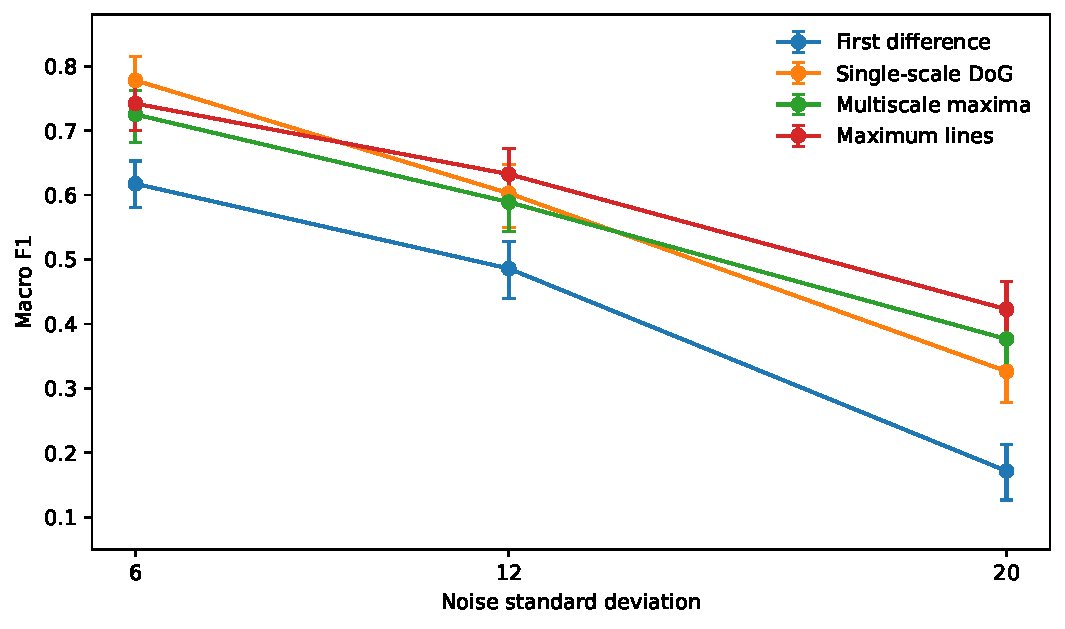
\includegraphics[width=0.82\textwidth]{figures/f1_by_noise_en.pdf}
\caption{Macro F1 by noise level, with bootstrap intervals.}
\label{fig:noise-f1}
\end{figure}

At $\sigma=6$, single-scale DoG reaches .778, ahead of maximum lines (.742). At $\sigma=12$, maximum lines reach .632, ahead of DoG (.603). At $\sigma=20$, they reach .423, compared with .326 for DoG and .172 for first differences. Cross-scale persistence becomes useful when local extrema are unstable, but remains costly for short events.

\subsection{Targeted Ablation of the Maximum-Line Pipeline}

A separate experiment uses 300 new series: 90 for calibration and 210 for evaluation. Each variant is calibrated independently on all its candidates. Intervals are based on 2,000 paired bootstrap replicates at the ablation-series level, seed 20260806, conditional on that calibration. They are exploratory and unadjusted for the fifteen pairwise contrasts among variants.

\begin{figure}[H]
\centering
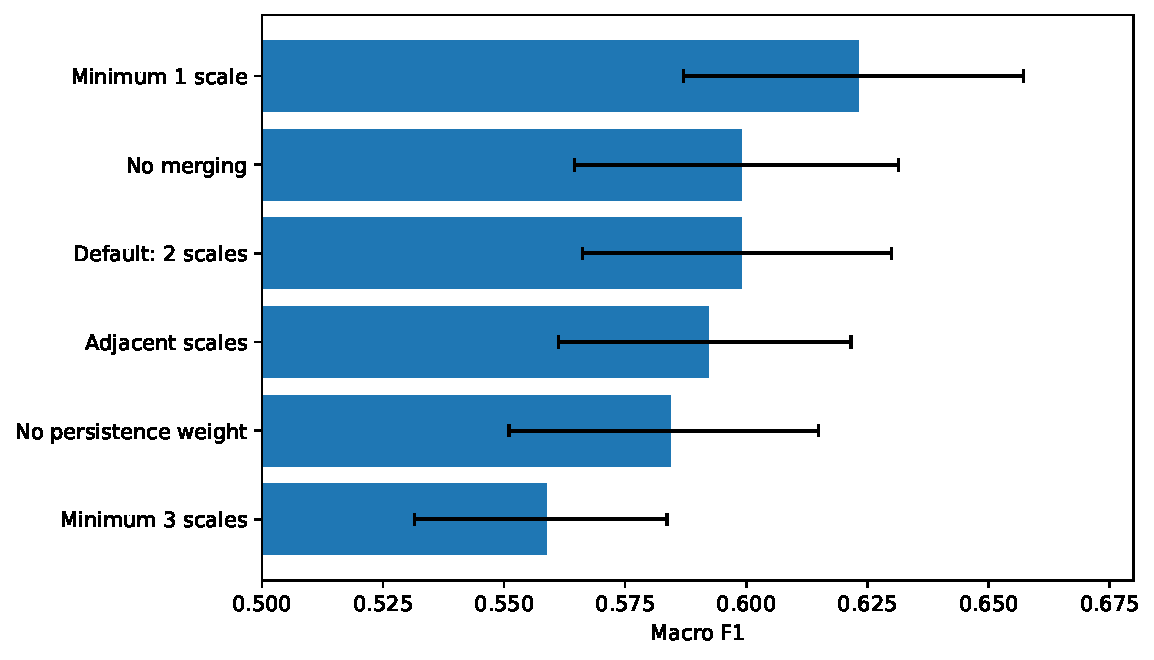
\includegraphics[width=0.88\textwidth]{figures/wtmm_ablation_en.pdf}
\caption{Macro F1 of maximum-line extractor variants on the ablation corpus.}
\label{fig:ablation}
\end{figure}

\begin{table}[H]
\centering
\caption{Targeted ablation with paired bootstrap intervals.}
\small
\begin{tabularx}{\textwidth}{@{}Xrrrr@{}}
\toprule
Variant & Macro P & Macro R & Macro F1 [95\% CI] & events/series \\
\midrule
Minimum 1 scale & .686 & .589 & \textbf{.623} [.587;.657] & 89.1 \\
No merging & .765 & .518 & .599 [.565;.631] & 50.7 \\
Default, minimum 2 scales & .713 & .528 & .599 [.566;.630] & 50.0 \\
Strictly adjacent scales & .701 & .523 & .592 [.561;.622] & 49.7 \\
No persistence weighting & .681 & .530 & .584 [.551;.615] & 50.0 \\
Minimum 3 scales & .681 & .483 & .559 [.532;.584] & 33.8 \\
\bottomrule
\end{tabularx}
\end{table}

